\documentclass{beamer}
\usepackage[utf8]{inputenc}
\usepackage{listings}
\usepackage{booktabs}
\usepackage{amssymb}
\usepackage{nicefrac}
\usepackage{amsmath}
\usepackage{bbm}
\usepackage{bm}
\usepackage{enumitem}
\usepackage{hyperref}
\usepackage[export]{adjustbox}
\usepackage{svg}

\usetheme{Madrid}
\definecolor{mlpblue}{rgb}{0.1, 0.14, 0.24}

\useoutertheme{infolines} % Alternatively: miniframes, infolines, split
\useinnertheme{circles}
\usecolortheme[named=mlpblue]{structure}

\DeclareMathOperator{\Tr}{Tr}
\DeclareMathOperator{\Cov}{Cov}
\DeclareMathOperator{\Concat}{Concat}

\DeclareMathOperator*{\argmax}{arg\,max}
\DeclareMathOperator*{\argmin}{arg\,min}
\DeclareMathOperator*{\indep}{\perp \!\!\! \perp}

\lstset{basicstyle=\footnotesize\ttfamily,breaklines=true}

%------------------------------------------------------------
%This block of code defines the information to appear in the
%Title page
\title[World Foundation Model Platform for Physical AI]{COSMOS}

\subtitle{Visuomotor Policy Learning via Action Diffusion} %\thanks{Beaglehole, Súkeník et.~al.~[NeurIPS 2024]}}

\author[MLP]{A. Buynitsky} 

\date{Nov 7, 2024}

\titlegraphic{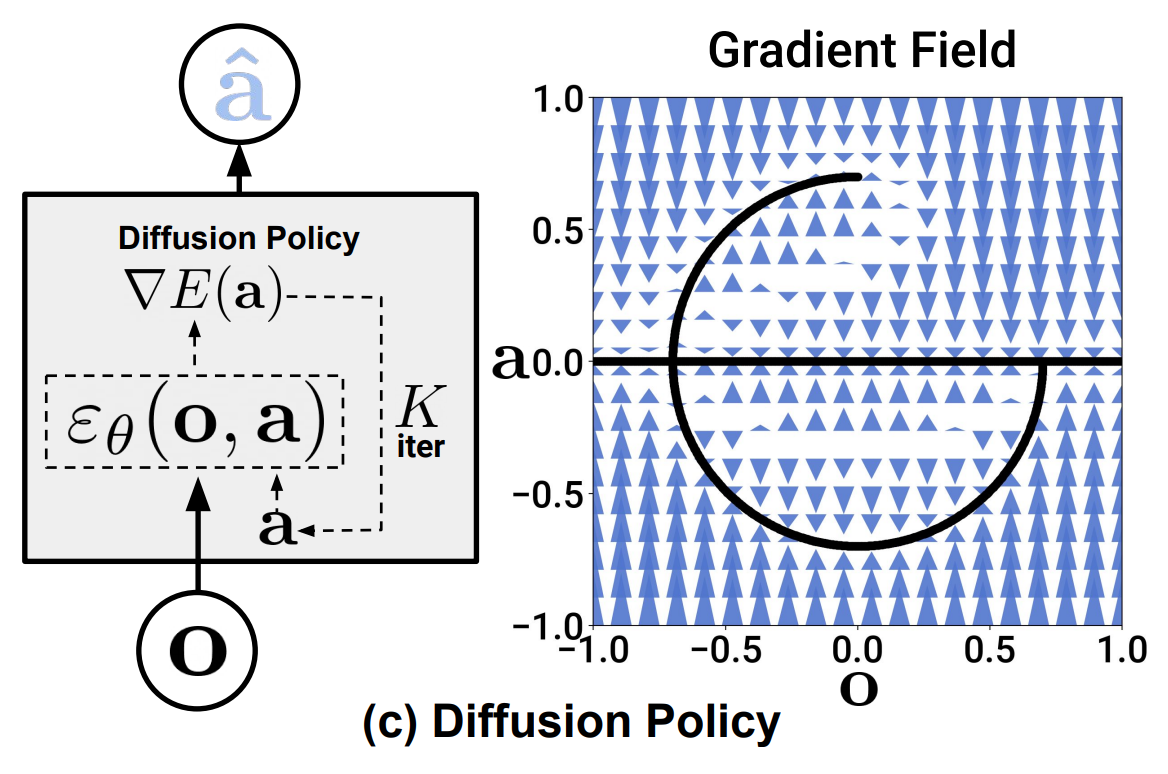
\includegraphics[width=5cm]{./img/diffusion_policy.png}}

%End of title page configuration block
%------------------------------------------------------------

%The next block of commands puts the table of contents at the 
%beginning of each section and highlights the current section:

\AtBeginSection[]
{
  \begin{frame}
    \frametitle{Outline}
    \tableofcontents[currentsection]
  \end{frame}
}
% ------------------------------------------------------------


\begin{document}

\frame{\titlepage}


%---------------------------------------------------------
% This block of code is for the table of contents after
% the title page
\begin{frame}
\frametitle{Outline}
\tableofcontents
\end{frame}
%---------------------------------------------------------
\section{TLDR}
\begin{frame}[t]{TLDR}
    \textbf{High Level:} Learn visuomotor policy through a diffusion process \newline
    \textbf{Results:} 46.9\% average improvement across 12 tasks (sim + real life)
    \begin{columns}
		\begin{column}{.5\textwidth}
			\begin{center}
				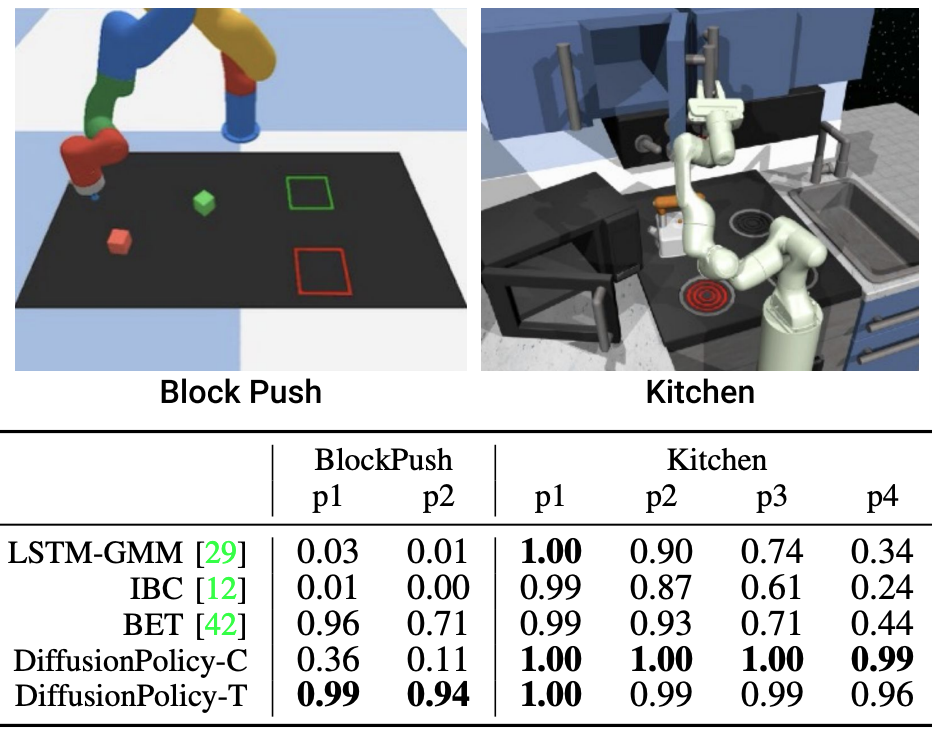
\includegraphics[width=\textwidth]{./img/dp_results.png}
			\end{center} \pause
		\end{column}
		\hspace{1em}
		\begin{column}{.5\textwidth}
            \textbf{Research Group:} Shuran Song; MIT, Columbia and Toyota Research Institute (TRI)\newline \pause
            \textbf{Future Work:}
            \begin{itemize}[label=-]
                \item Apply Diffusion Policy to RL to avoid suboptimal data
                \item Accelerate inference time + decrease computational costs with advancements from modern diffusion methods
            \end{itemize}
		\end{column}
	\end{columns}
\end{frame}


\section{Related Work}

\begin{frame}[t]{BC-RNN / LSTM-RNN}
    \textbf{Behavioral Cloning} learns a policy $\pi_\theta(s)$ to clone actions from a set of demonstrations:
    \[
    \mathop{\arg \min}\limits_{\theta} \mathbb{E}_{(s,a) \sim \mathit{D}} || \pi_\theta(s) - a||^2
    \]
    \newline
    \pause
    \textbf{Method:}
    \small
    \begin{itemize}[label=-]
      \item RNN models temporal dependencies $(s_t, a_t, \dots, s_{t+T},a_{t+T})$ via hidden state
      \item predicts the sequence of action and is unrolled one step at a time: \[a_t, h_{t+1} = \pi_\theta(s_t, h_t)\]
    \end{itemize}
    
    \normalsize
    \begin{columns}
        \hspace{1em}
		\begin{column}{.8\textwidth}
            %\textbf{Data Collection}
            %\begin{enumerate}[label=\arabic*.]
            %    \small
            %    \item Machine-Generated
            %    % RL Algorithm takes agent checkpoints and collects 300 rollouts from each
            %    % mixture of expert and suboptimal data
            %    \item Human-Generated
            %    % proficient human: collected by humans through teleopp platform
            %    % multi-human: 300 demos by 6 teleoperations of varying proficiency
            %    \item Observation Modalities
            %    % capture diverse set of sensor streams (end-effector, gripper fingers, joins) + camera and images
            %    \normalsize
            %\end{enumerate}
            \pause
            \textbf{Limitation}
            \begin{enumerate}[label=\arabic*.]
                \item Biased towards one mode
                \item Brittle performance due to changes in observation space and hyperparameters
            \end{enumerate}
		\end{column}
        \hspace{-1em}
		\begin{column}{.2\textwidth}
            \begin{center}
                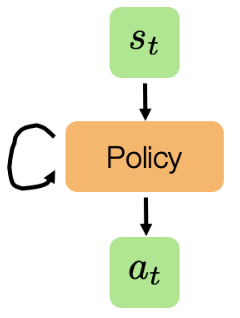
\includegraphics[width=\textwidth]{./img/bc_rnn.png}
            \end{center}
		\end{column}
        \hspace{2em}
	\end{columns}

    % \textbf{Conclusions}
    % \begin{enumerate}[label=\arabic*.]
    %     \small
    %     \item Observation history crucial for good performance
    %     % BC-RNN + BC significantly improve perf over long horizon tasks
    %     \item Variance in demonstration quality
    %     % trajectory length noise in robot movement/mistakes
    %     \item dataset size
    %     % offline policy sensitive to state + action space and dataset size
    %     \normalsize
    % \end{enumerate}

        % challenges: data from 
\end{frame}

\begin{frame}[t]{Behavior Transformer (BET)}
    \textbf{Large Scale} human datasets have wide variances with multiple modes
    \begin{center}
        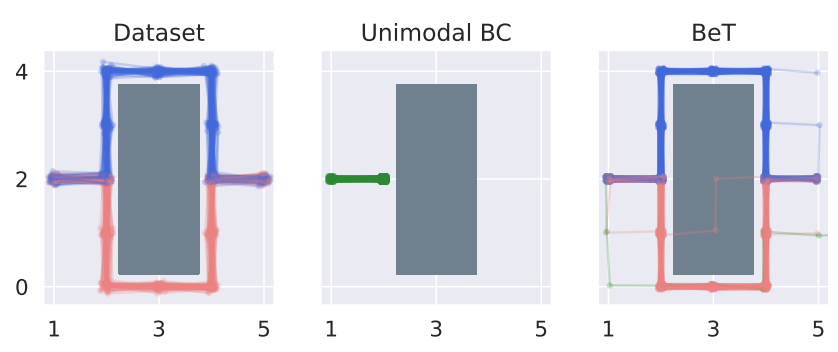
\includegraphics[width=0.8\textwidth]{./img/bet.png}
    \end{center}
    \textbf{Limitation of BC:} Current bc assumes that data is drawn from unimodal experts solving a single task
    % current bc methods assume that data is drawn from unimodal experts solving a single task
    % current policies are goal conditions where each goal implies a single mode of behavior
    % BH datasets have wide variances,m multiple modes + human demos do not come with reward labels
    % limit applicaiton of current methods in offline Rl + BC from datasets
\end{frame}

\begin{frame}[t]{Behavior Transformer (BET)}
	\begin{columns}
        \hspace{1em}
		\begin{column}{0.4\textwidth}
            \textbf{Propossed Solution:}
            \begin{enumerate}[label=\arabic*.]
                \item Descretize action dataset into $k$ bins with k-means with offset
                \item Train a transformer with two heads to predict an action bin and an offset for that bin
            \end{enumerate}
		\end{column}
		\begin{column}{0.6\textwidth}
            \begin{center}
                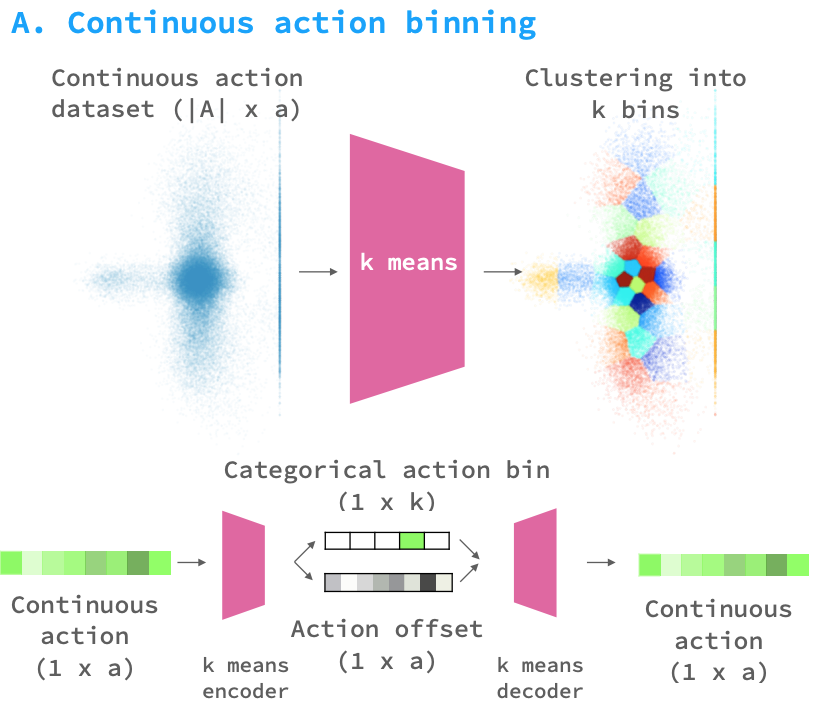
\includegraphics[width=0.7\textwidth]{./img/bet_action.png}
            \end{center}
		\end{column}
	\end{columns}
    \pause
    \vspace{-0.5em}
    \textbf{Inference:}
    \begin{center}
        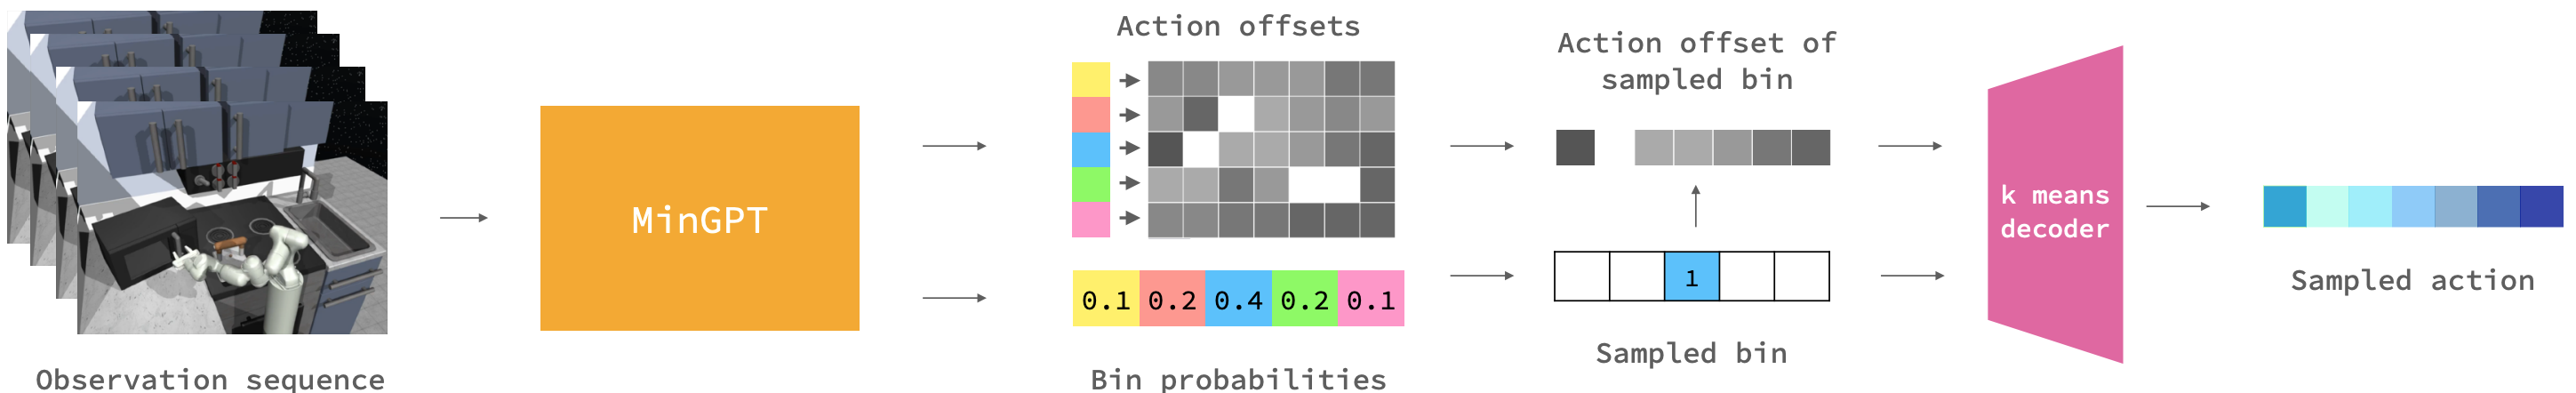
\includegraphics[width=\textwidth]{./img/bet_inference.png}
    \end{center}
    \pause
    \vspace{-0.5em}
    \textbf{Limitation:} Inconsistent sampling from action bins
\end{frame}


\begin{frame}[t]{Implicit BC}
	\begin{columns}
        \hspace{1em}
		\begin{column}{0.5\textwidth}
            \textbf{BC Reformulation:} Use Energy-Based models instead of explicit policies \newline
            \newline
            \textbf{Energy Models:} Scalar energy function captures the relationship between states and actions
		\end{column}
		\begin{column}{0.5\textwidth}
            \begin{center}
                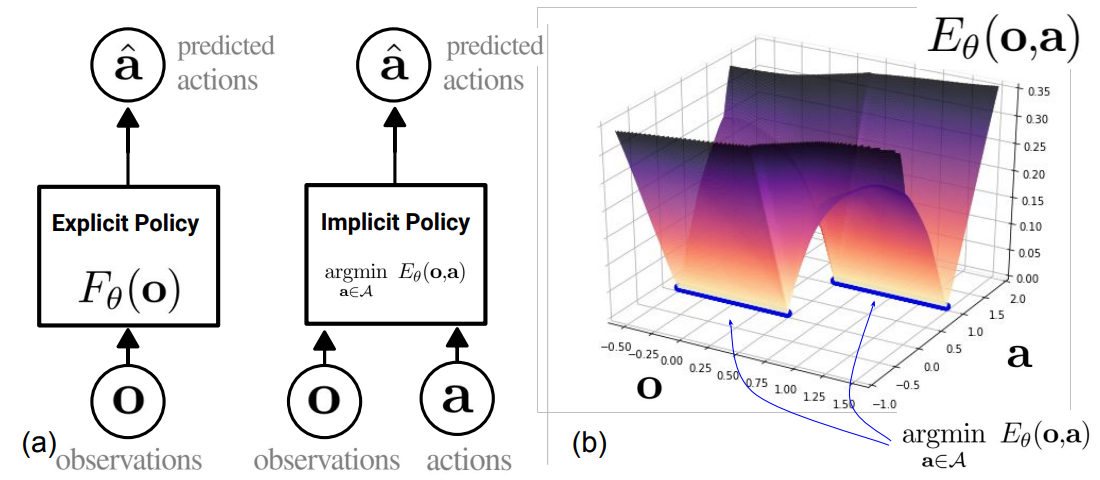
\includegraphics[width=\textwidth]{./img/ebm.png}
            \end{center}
		\end{column}
    \hspace{2em}
	\end{columns}
    \vspace{1em}
    \pause
    \textbf{Inference}: solve optimization problem (i.e. with gradient descent) for:
    \[
    %\hat{a} = argmin \limits_{a \in A} E_\theta (o,a) \hspace{1em}
    \hat{a} = \mathop{\arg \min}\limits_{a \in A} \mathbf{E}(o,a)
    \]
    \pause
    \textbf{Limitation}: Increases complexity, training and inference time, and computational cost 

    % learn loss using negative log-likelihood loss fn
    % assigns low energy values to more probable / desired configs
    % higher energy value to les pourable / undesirable configs
    % capture the relationship between states and actions
    % optimizes for optimal action via gradient descent
\end{frame}






\section{Background \& Intuition}

\begin{frame}{Learning}
    Assume that all Data (image, speech, etc.) is sampled from a distribution \newline \newline \pause 
    \textbf{Generative Model:} learn training distribution $P_{\theta}(x)$ from dataset
	\begin{columns}
		\begin{column}{.5\textwidth}
			\begin{center}
                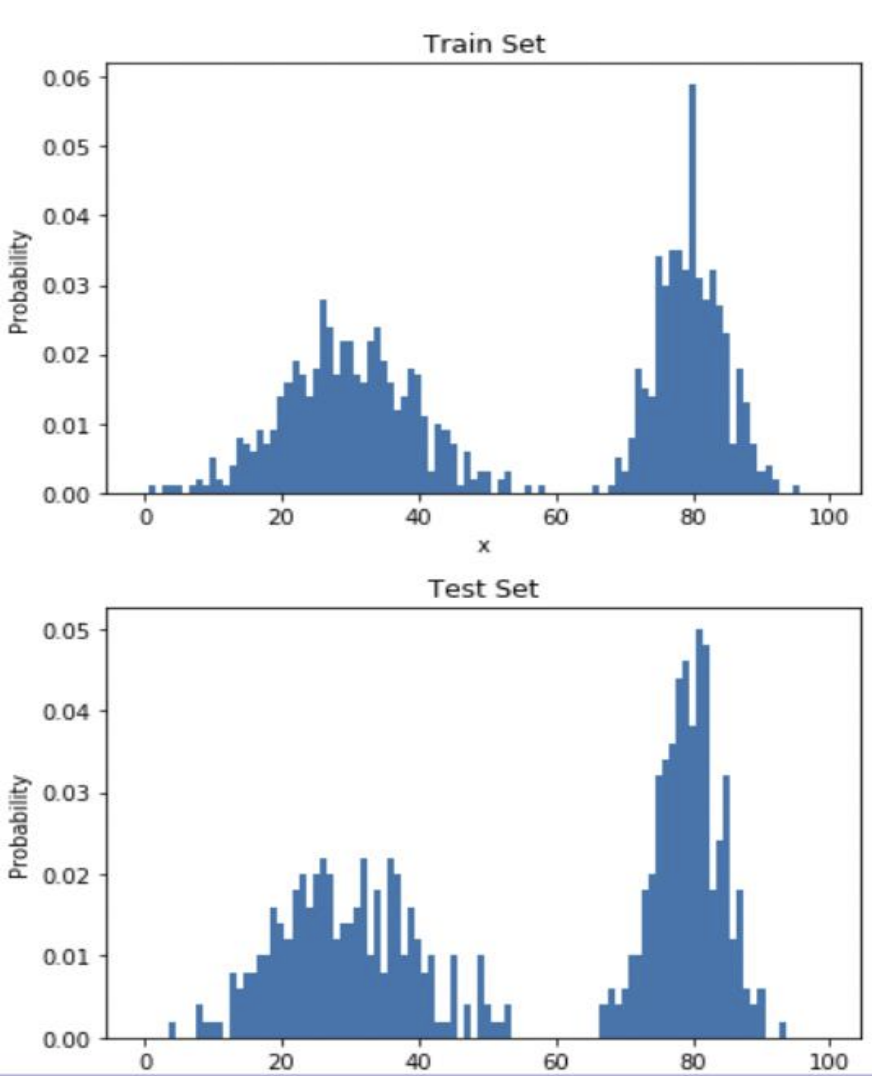
\includegraphics[width=0.8\textwidth]{./img/distribution.png}
			\end{center} \pause
		\end{column}
		\hspace{0.5em}
		\begin{column}{.5\textwidth}
            \textbf{Diffusion Models} model the output as a denoising process, 
            performing $T$ denoising steps to produce a series of intermediate actions with decreasing noise levels.
		\end{column}
		\hspace{0.5em}
	\end{columns}
\end{frame}

\begin{frame}[t]{Diffusion Overview (Forward Process)}
    \begin{center}
        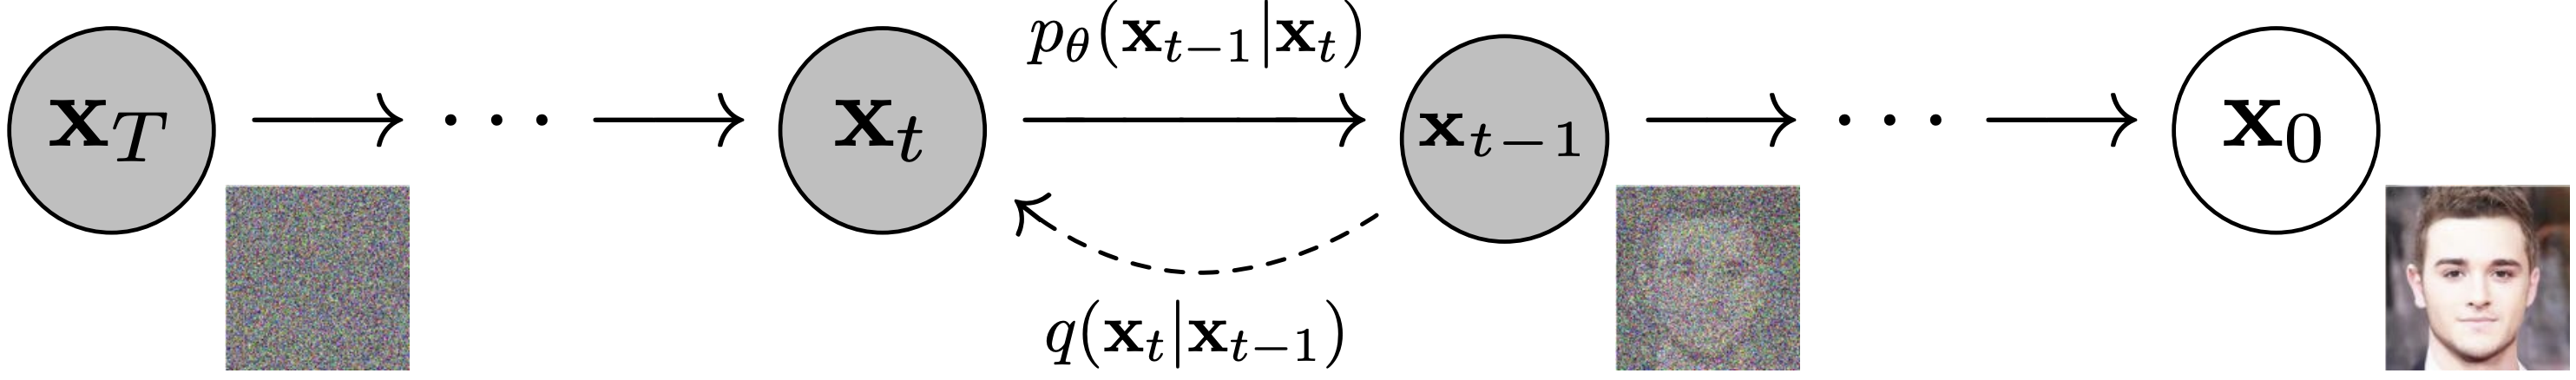
\includegraphics[width=.9\textwidth]{./img/img_diffusion.png}
    \end{center}
    \textbf{Forward Process ($q(x_t \mid x_{t-1})$):} Markov chain that gradually adds \\ \hspace{1em} Gaussian Noise according to variance schedule $\beta_t \in [\beta_1, \dots, \beta_T]$
    % x_1 ... x_t are patients of the same dimensionality as the data
    % forward process variances B_t can either be learned or held constant 
    \[
    q(x_{1:T} \mid x_0) := \prod_{t=1}^{T} q(x_t \mid x_{t-1}),\hspace{1em} q(x_t \mid q_{t-1}) := \mathbf{N}(x_t; \sqrt{1 - \beta_t} x_{t-1}, \beta_T \mathbf{I})
    \] \\ \pause
    \textbf{Reparametrization for $q(x_t \mid x_0)$} allows for sampling $x_t$ at arbitrary $t$:

    \[
    q(x_t \mid x_0) = N(x_t; \sqrt{\bar{\alpha}_t}x_0, (1-\bar{\alpha}_t)\mathbf{I}) \hspace{1em} \text{where:}
    \]
    \[
    \bar{\alpha}_t := \prod_{s=1}^t \alpha_s \hspace{1em} \text{and}\hspace{1em} \alpha_s = 1 - \beta_t
    \]
\end{frame}

\begin{frame}{Diffusion Overview (Backward Process)}
    \begin{center}
        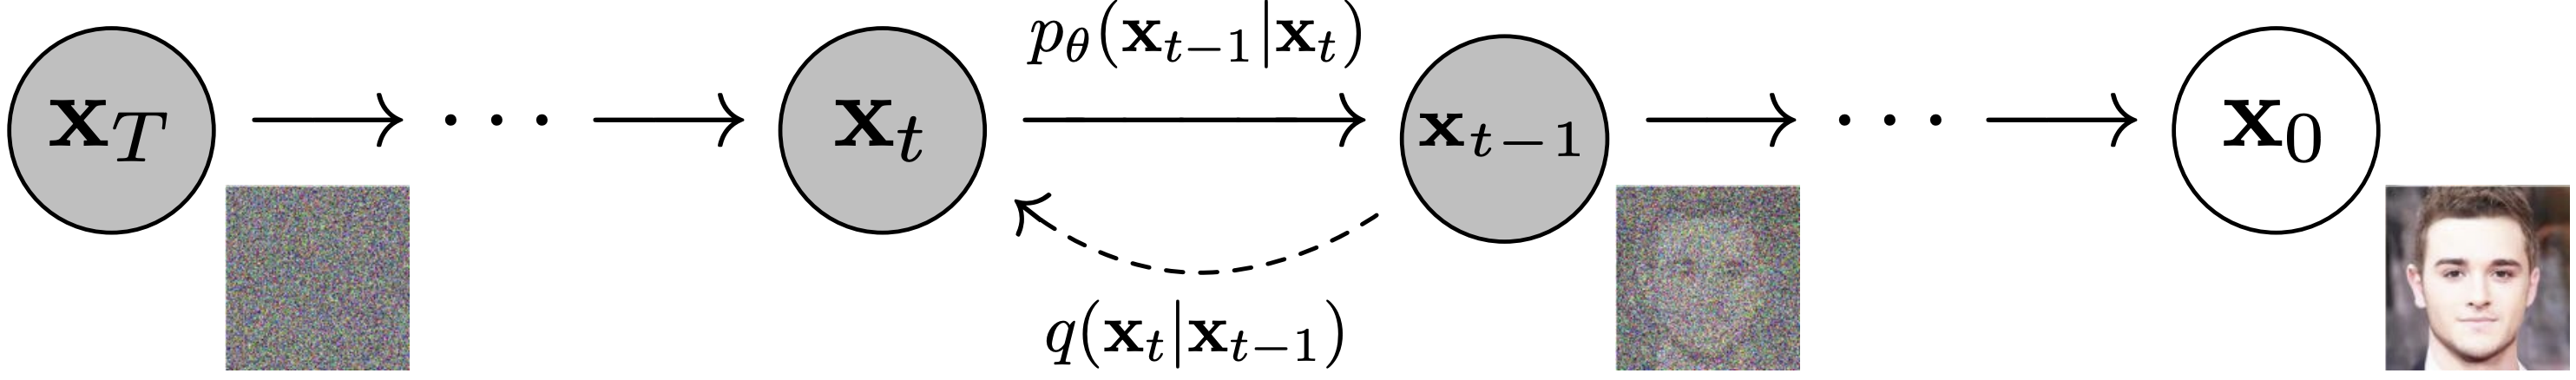
\includegraphics[width=.9\textwidth]{./img/img_diffusion.png}
    \end{center}
    \textbf{Backward Process ($p_\theta(x_{t-1} \mid x_{t})$):} Markov chain with learned Gaussian \\ \hspace{1em} transitions initialized with $p(x_T) = \mathbf{N}(x_T; 0, \mathbf{I})$
    \begin{gather}
    p_{\theta}(x_{0:T}) := p(x_t)\prod_{t=1}^{T} p_{\theta}(x_{t-1} \mid x_{t})
    \\
    p_\theta(x_{t-1} \mid x_t):= \mathbf{N}(x_{t-1}; \mu_\theta(x_t, t), \Sigma_\theta(x_t,t))
    \end{gather}
    \newline
    $\Sigma_\theta(x_t,t) = \sigma_t^2 \mathbf{I}$: Fix to untrained time dependent constants (i.e. $\sigma_t^2 = \beta_t$)\newline \newline
    $\mu_\theta(x_t,t)$: Reparametrize to predict the noise at step $t$ with $\epsilon_\theta (x_t, t)$ \newline \newline \pause
\end{frame}

\begin{frame}{Diffusion Overview (Backward Process)}
    \begin{center}
        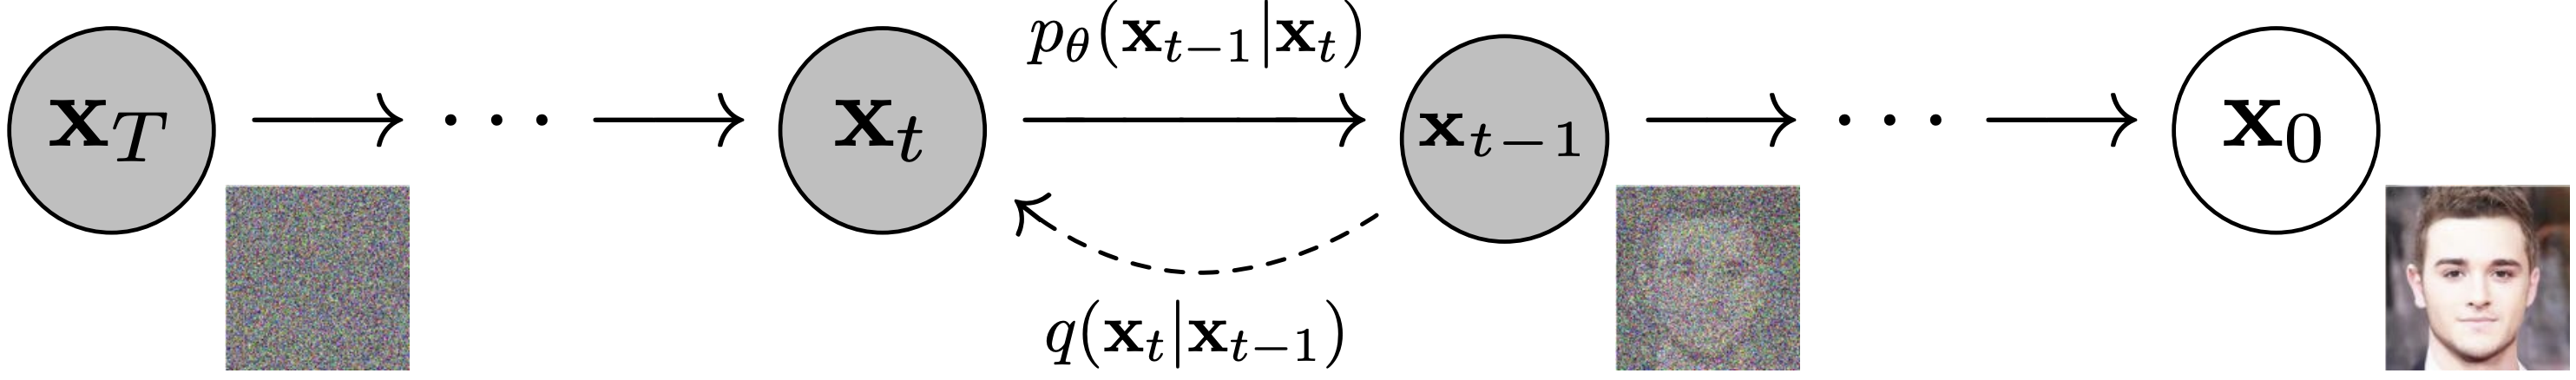
\includegraphics[width=.9\textwidth]{./img/img_diffusion.png}
    \end{center}
    \textbf{Backward Process ($p_\theta(x_{t-1} \mid x_{t})$):} Markov chain with learned Gaussian \\ \hspace{1em} transitions initialized with $p(x_T) = \mathbf{N}(x_T; 0, \mathbf{I})$ \newline \newline
    $T$ Denoising iterations performed with decreasing levels of noise producing: \\ \hspace{1em} $x_T, x_{T-1}, \dots, x_0$ following:
    \begin{gather}
    x_{t-1} = \alpha(x_t - \gamma \epsilon_\theta(x_t, t) + \textbf{N}(0, \sigma^2, I))\label{eq:1}
    \end{gather}
    Above can be interpreted as a single noisy gradient step:
    % if drop the alpha (alpha < 1) will increase straning
    % the N will be from the normal distribution training
    \[
    x' = x - \gamma \nabla E(x)
    \]
    Where $\epsilon_\theta(x, t)$ predicts $E(x)$ with learning rate $\gamma$ and parameters $\alpha$ and $\sigma^2$
\end{frame}

\begin{frame}[t]{Diffusion Training}
    \begin{center}
        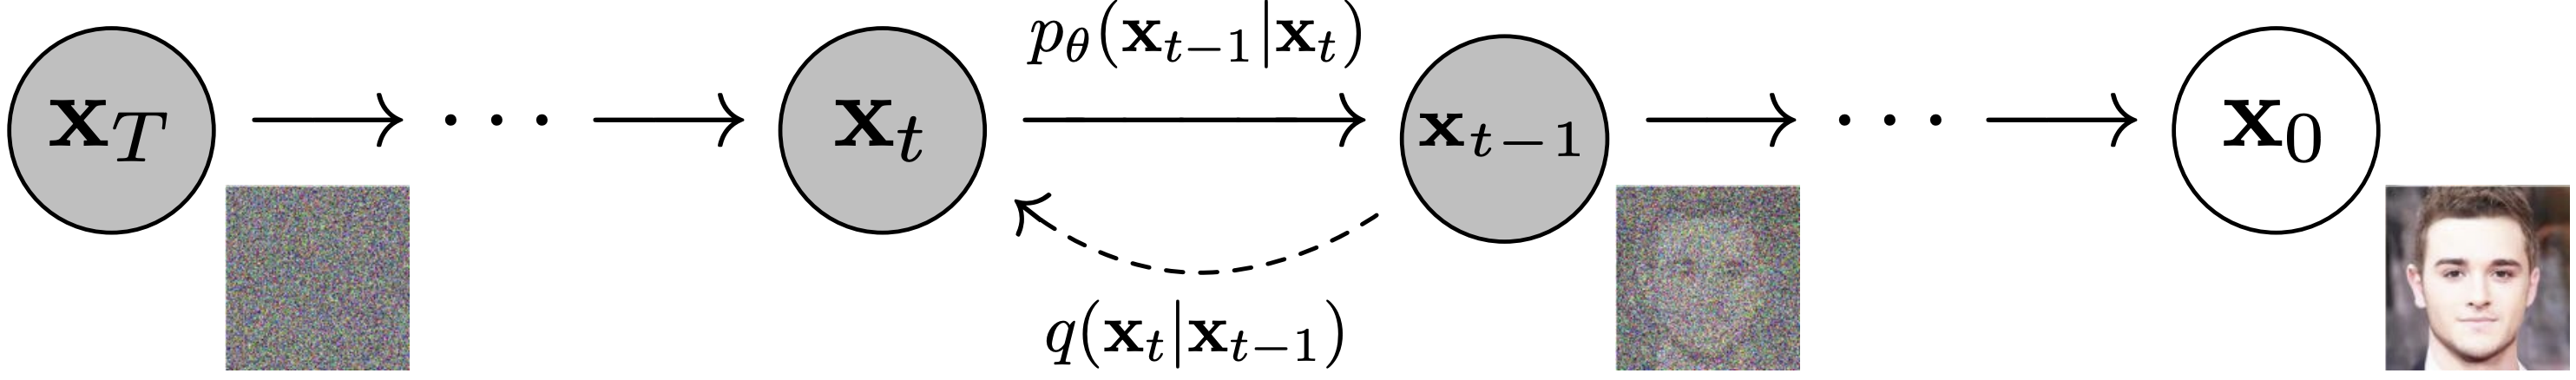
\includegraphics[width=.9\textwidth]{./img/img_diffusion.png}
    \end{center}
    \begin{enumerate}[label=\arabic*.]
        \item Randomly sampling examples $x_0$ from training dataset \pause
        \item For each sample randomly select denoising iteration $k \in [1, \dots, T]$ \\ \hspace{1em} and noise $\epsilon_k$ with appropriate variance for $k$ \pause
        \item  Noise Prediction Network $\epsilon_\theta$ predicts noise from noisy data:
        \begin{gather}\label{eq:2}
            \mathcal{L} = MSE(\epsilon_k, \epsilon_\theta(x_0 + \epsilon_k, k))
        \end{gather}
    \end{enumerate}
\end{frame}

\section{Diffusion for Visuomotor Policies}
\begin{frame}[t]{Modifying Image Diffusion to Robotic Diffusion}
    % temporal consistency + smoothness in long-horizon planning conditioned on observations
    % action-sequence prediction with receding horizon control
    \textbf{Action Sequence Prediction:} 
    \begin{itemize}[label=-]
        \item At step $t$ policy takes latest $T_o$ steps of observation data $O_t$
        \item Policy predicts $T_p$ action steps
        \item The first $T_a$ of $T_p$ steps are executed
    \end{itemize}
    \begin{center}
    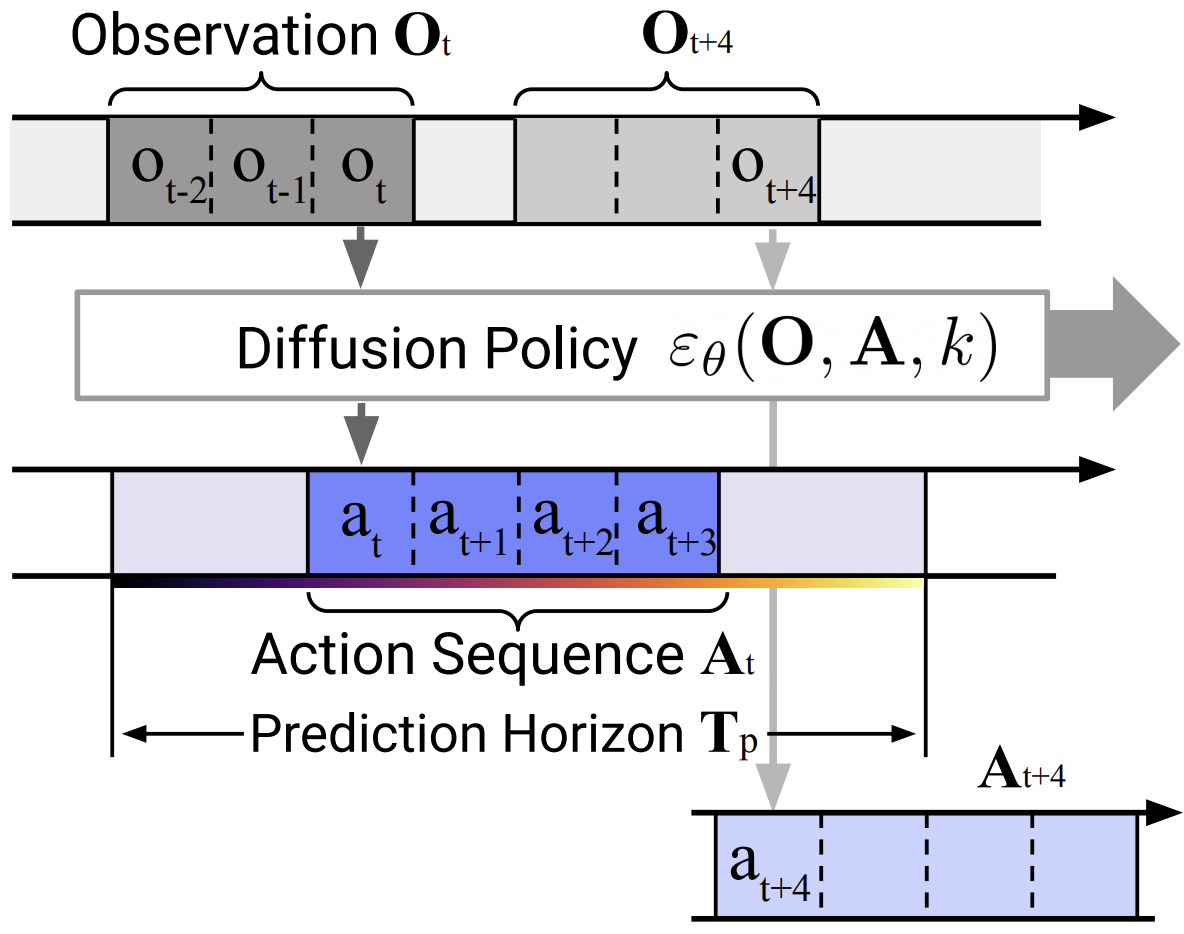
\includegraphics[width=0.5\textwidth]{./img/diffusion_overview.png}
    \end{center}
    % Speed up diffusion processes by learning

    % excluding O_t prediction enables end-to-end training of vision encoder feasible
\end{frame}
\begin{frame}[t]{Modifying Image Diffusion to Robotic Diffusion}
    \textbf{Visual Observation Conditioning:} 
    Learn conditional distribution $p(A_t \mid O_t)$ instead of joint distribution $p(A_t, O_t)$
    \newline
    \newline
    Modify denoising iterations \eqref{eq:1} to:
    \[
    A_t^{k-1} = \alpha(A_t^k - \gamma \epsilon_\theta (O_t, A_t^k, k) + \textbf{N}(0, \sigma^2, I))
    \]
    Modify MSE Loss \eqref{eq:2} to:
    \[
        \mathcal{L} = MSE(\epsilon_k, \epsilon_\theta(O_t, A_t^0 + \epsilon^k, k))
    \]
    \begin{center}
        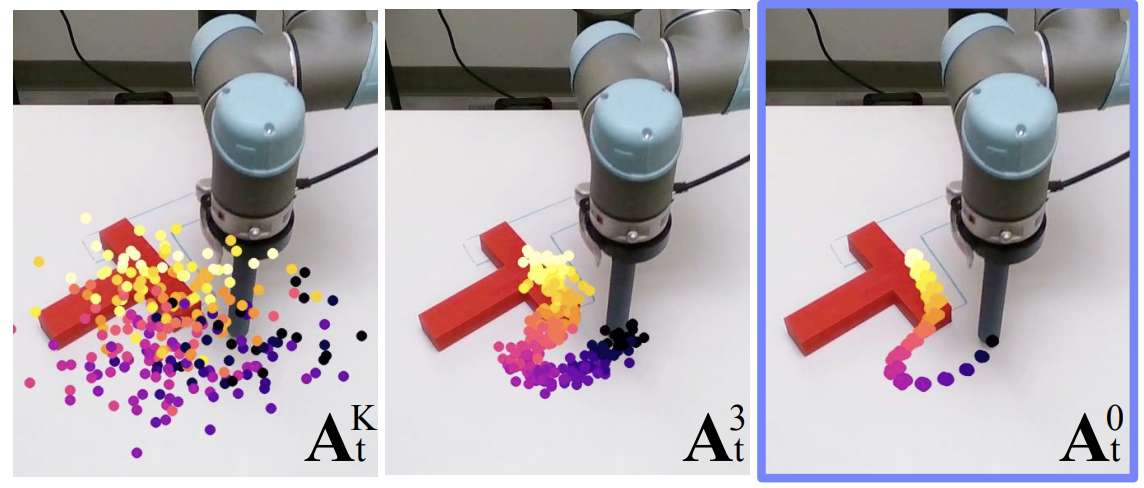
\includegraphics[width=0.7\textwidth]{./img/robotic_diffusion.png}
    \end{center}
    % excluding O_t prediction enables end-to-end training of vision encoder feasible
\end{frame}

\begin{frame}[t]{Vision Encoder}
    Choice of noise prediction network $\epsilon_\theta$ is \textbf{independent} of visual encoders
    Vision encoder maps raw image sequence to latent embedding $O_t$ from multiple camera views\\
    Use a standard \textbf{Resnet-18} with the following modifications:
    \begin{itemize}[label=-]
        \item Replace global average pooling with spatial softmax pooling
        % spatial softmax pooling 
        \item Replace BatchNorm with GroupNorm
        % batch normalizes by calculating mean + variance across all feature dimensions
        % gropu norm normalizs by dividing feature channels into groups and then normalizes the features in each group
    \end{itemize}
    \begin{center}
        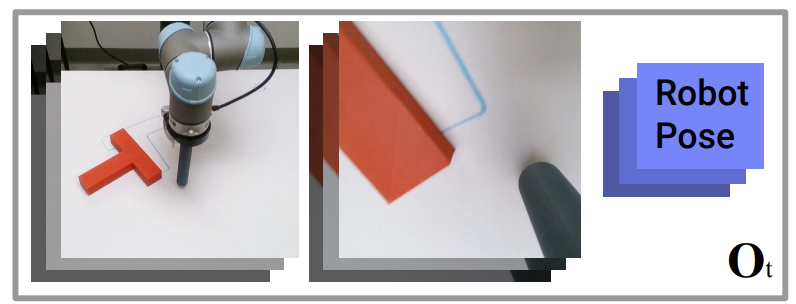
\includegraphics[width=0.7\textwidth]{./img/img_encoder.png}
    \end{center}
    End-to-end performs better than pre-trained vision encoders.
\end{frame}

\begin{frame}[t]{Option 1: CNN-Based Diffusion Policy}
    % temporal consistency + smoothness in long-horizon planning conditioned on observations
    % action-sequence prediction with receding horizon control
    % excluding O_t prediction enables end-to-end training of vision encoder feasible
    \textbf{1D temporal CNN:} learn training distribution $P_{\theta}(x)$ from dataset
    % 1D sequence data A_t
	\begin{columns}
		\begin{column}{.5\textwidth}
            \textbf{Method:}
            \begin{itemize}[label=-]
                \item Condition on $O_t$ using FiLM layers
                % FILM: apply a scale (a) and shift (b) to output features of conv layer
                % use a linear protecting to find a and b
                % applied independently to each feature
                \item Only Predict Action Trajectory 
            \end{itemize}
            \textbf{Result:}
            \begin{itemize}[label=-]
                \item Ok performance on most tasks 
                \item Poor performance when desired action sequence changes rapidly
            \end{itemize}
		\end{column}
		\begin{column}{.5\textwidth}
			\begin{center}
                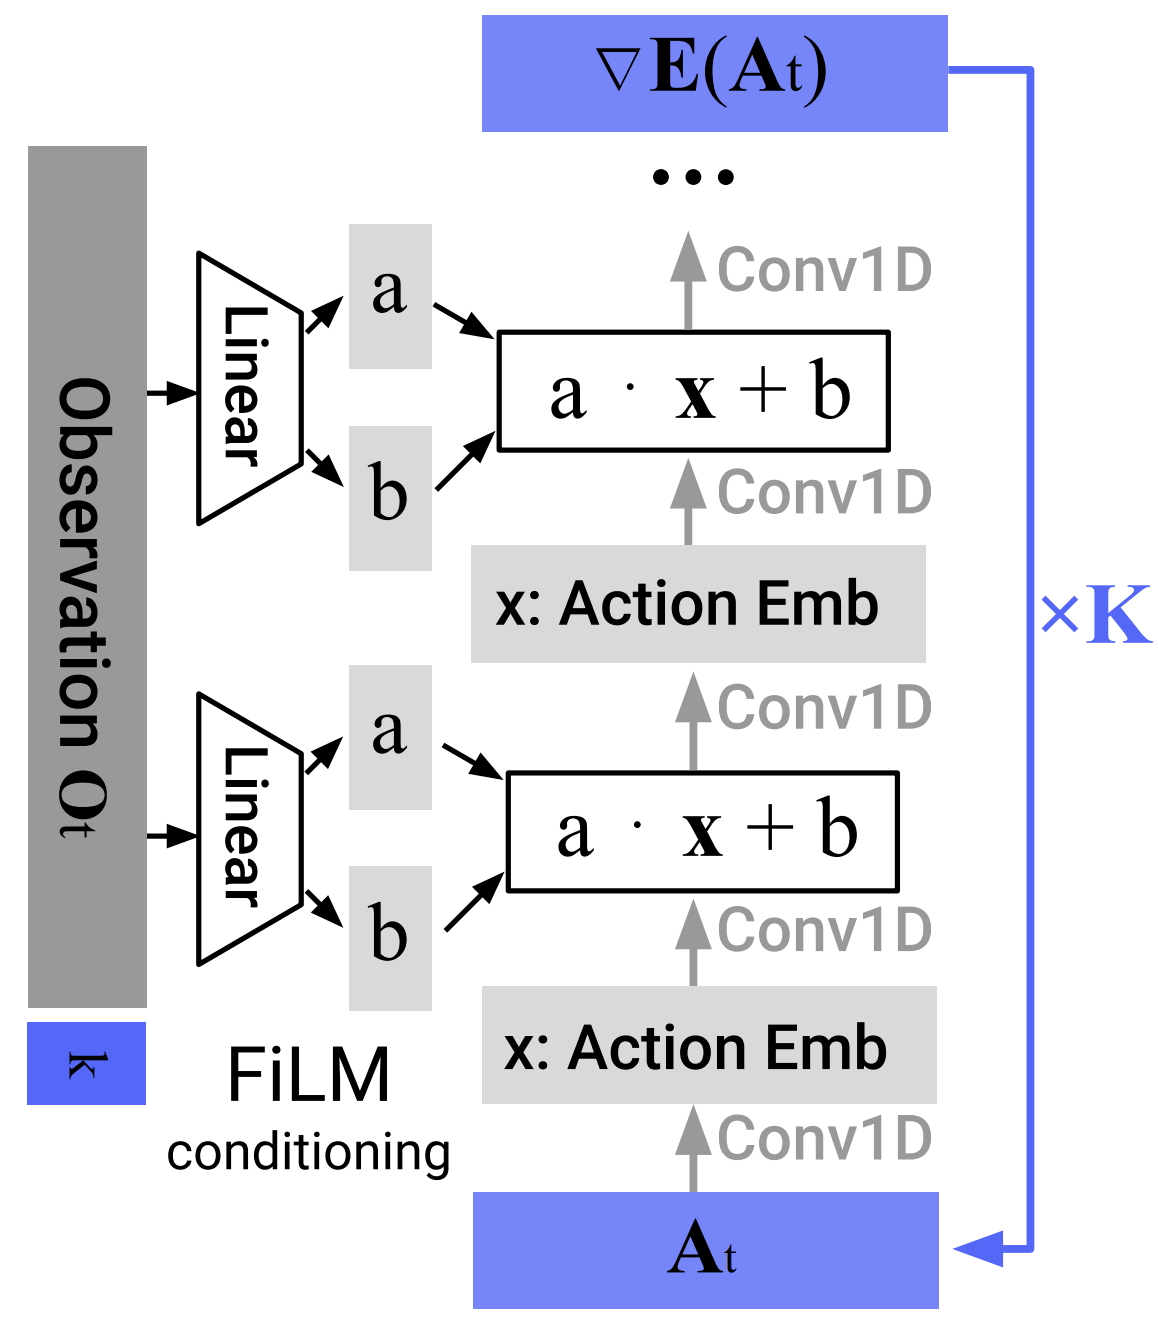
\includegraphics[width=0.95\textwidth]{./img/cnn_diffusion.png}
			\end{center}
		\end{column}
	\end{columns}
\end{frame}

\begin{frame}[t]{Option 2: Time-series Diffusion Transformer}
    \textbf{Time-Series Transformer:} Adopted from MinGPT 
	\begin{columns}
		\begin{column}{.5\textwidth}
            \textbf{Transformer Input:}
            \begin{itemize}[label=-]
                \item Noisy Actions $A_t^k$ 
                \item Embedding for diffusion iteration $k$
                \item Observations $O_t$ transformed into input tokens by MLP
            \end{itemize}
            \textbf{Result:}
            \begin{itemize}[label=-]
                \item Best performing policy on even complicated tasks
                \item  Sensitive to hyperparameter tuning
            \end{itemize}
		\end{column}
		\begin{column}{.5\textwidth}
			\begin{center}
                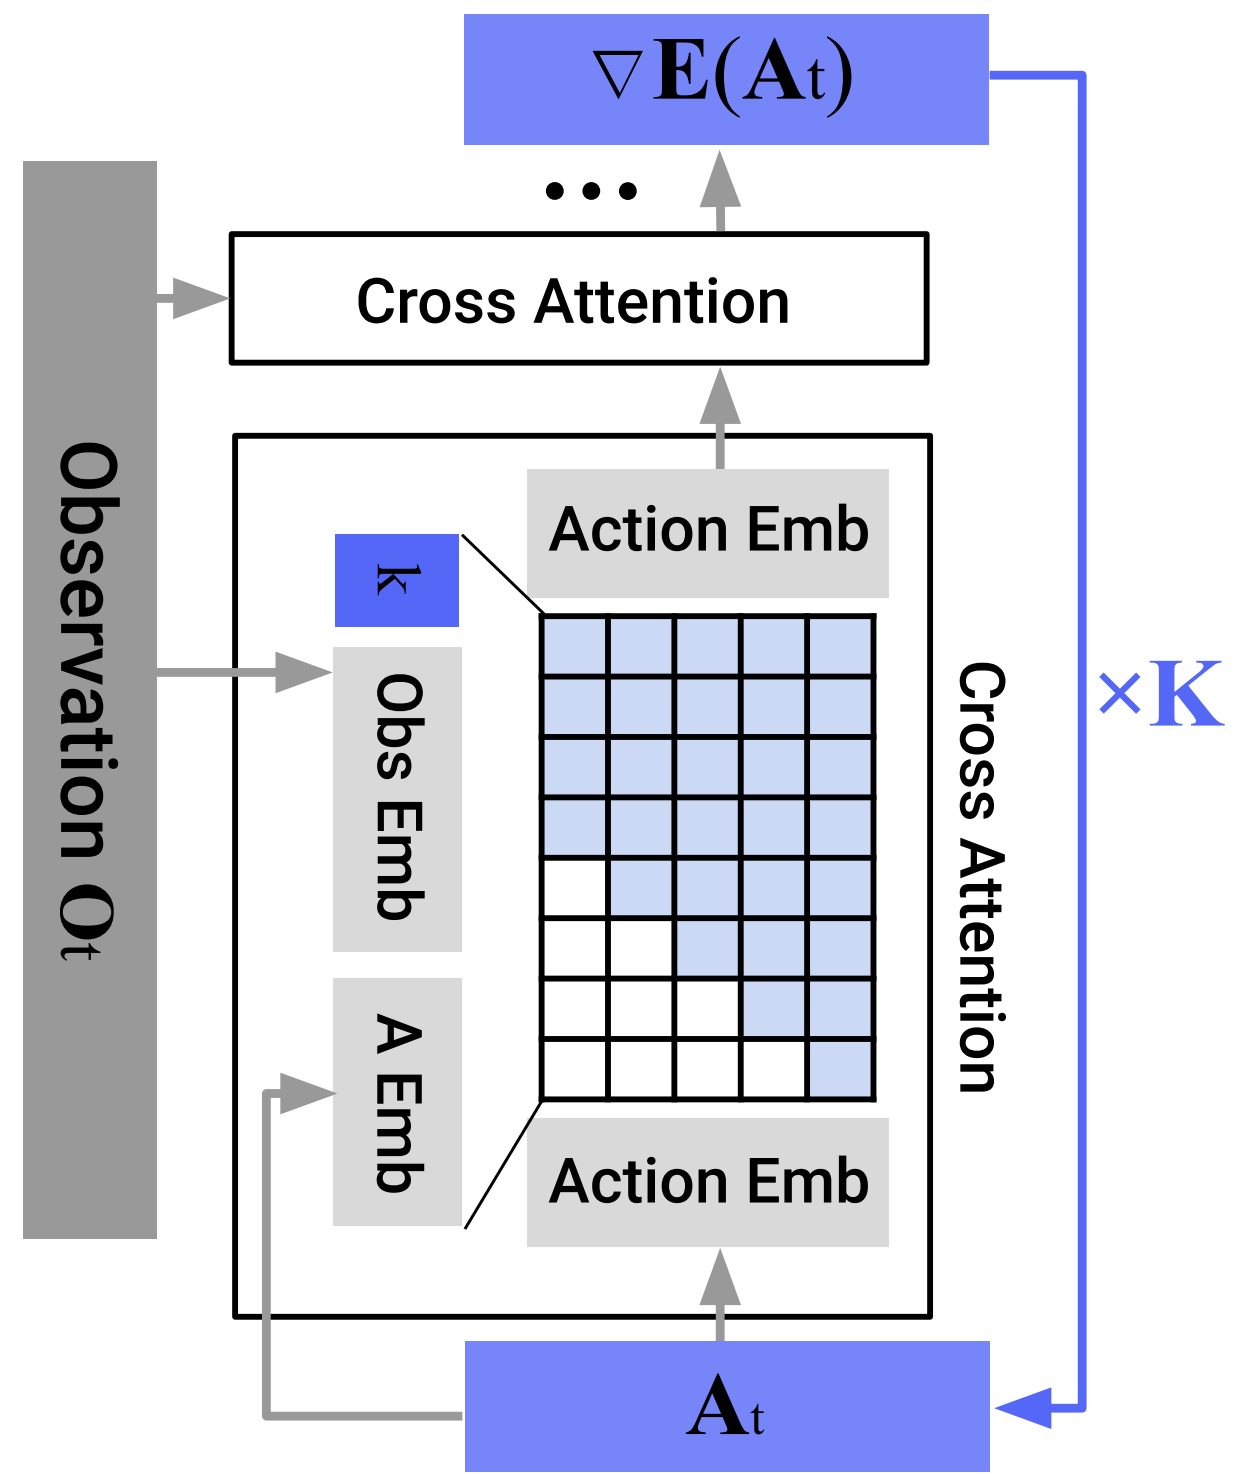
\includegraphics[width=0.95\textwidth]{./img/tft_diffusion.png}
			\end{center}
		\end{column}
	\end{columns}
\end{frame}

\begin{frame}[t]{Final Result:}
    \begin{center}
        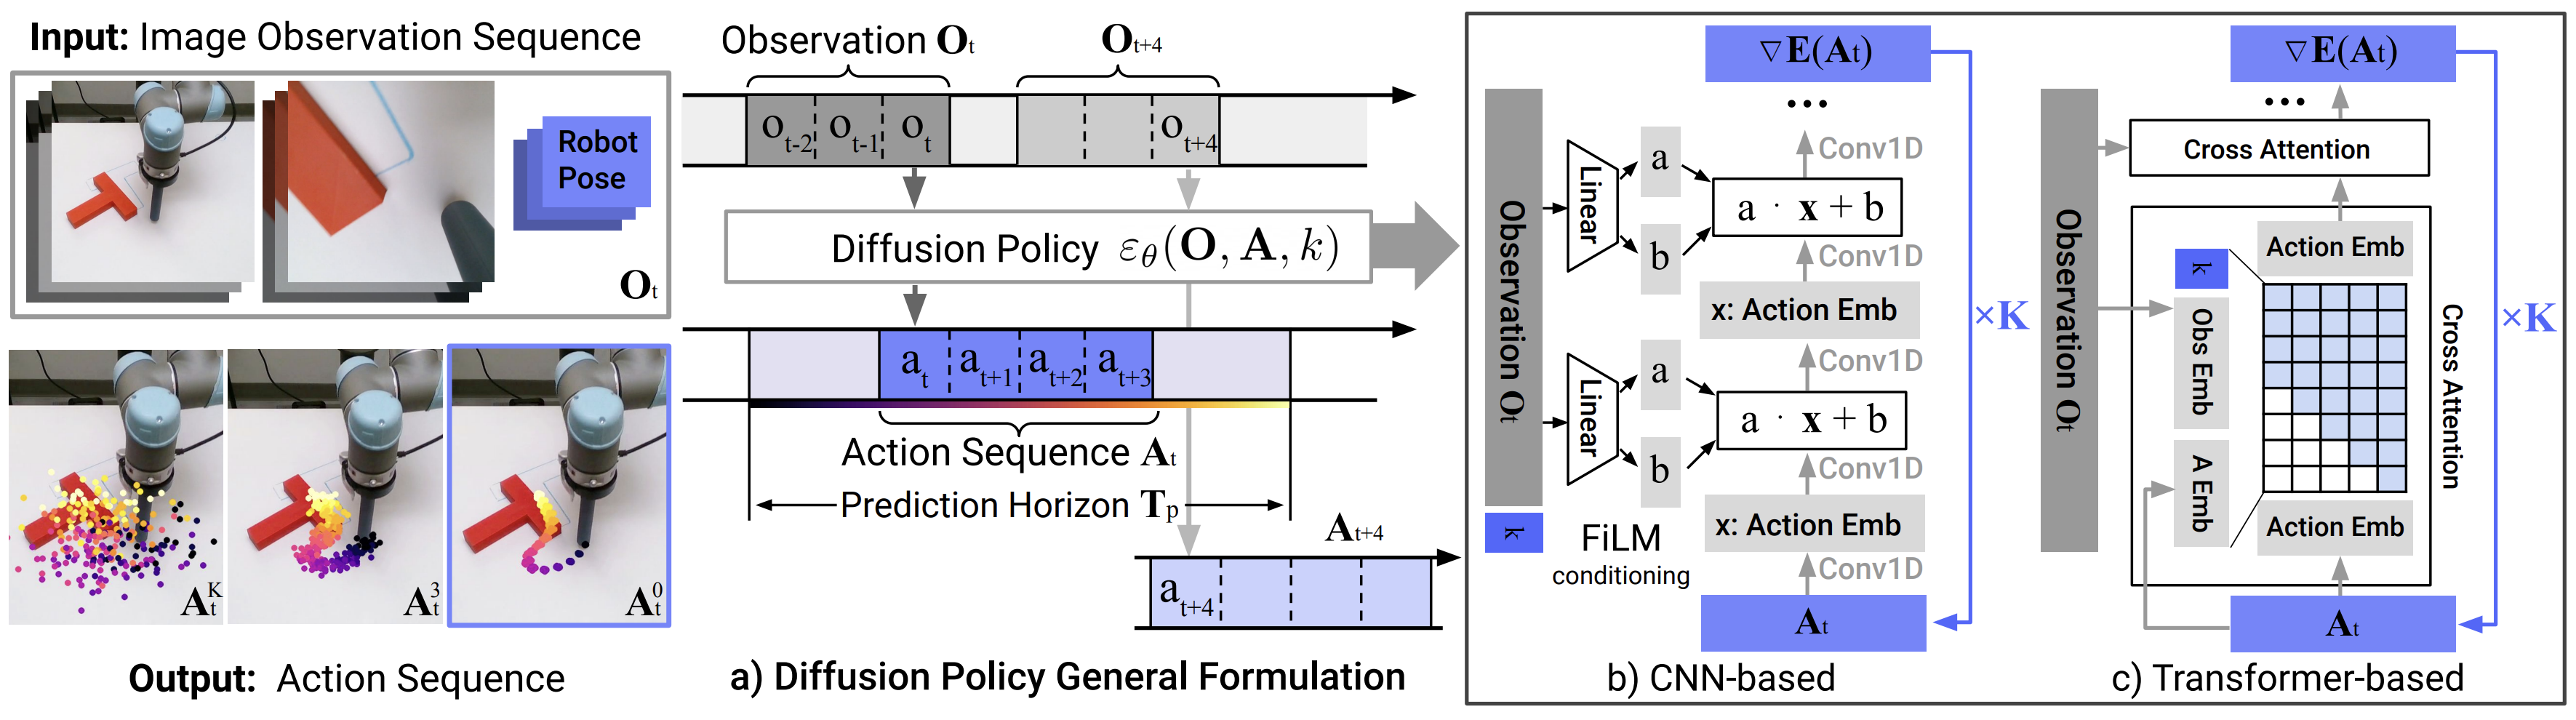
\includegraphics[width=0.95\textwidth]{./img/diffusion_result.png}
    \end{center}
\end{frame}

% inference: can be accelerated 10x by using fewer iterations for infernece speeds (0.1s latency)



\section{Diffusion Properties}
\begin{frame}[t]{Convergence Basins}
    \textbf{$A_t^K$ is stochastically initialized}:
    \begin{itemize}[label=-]
        \item Help specify different convergence basins for final action prediction $A_t^0$
    \end{itemize}
    
    \textbf{$A_t^K$ is stochastically pertubated}:
    \begin{itemize}[label=-]
        \item $K$ iterations enable individual action samples to converge and move between differnet action basins.
    \end{itemize}
    \begin{center}
        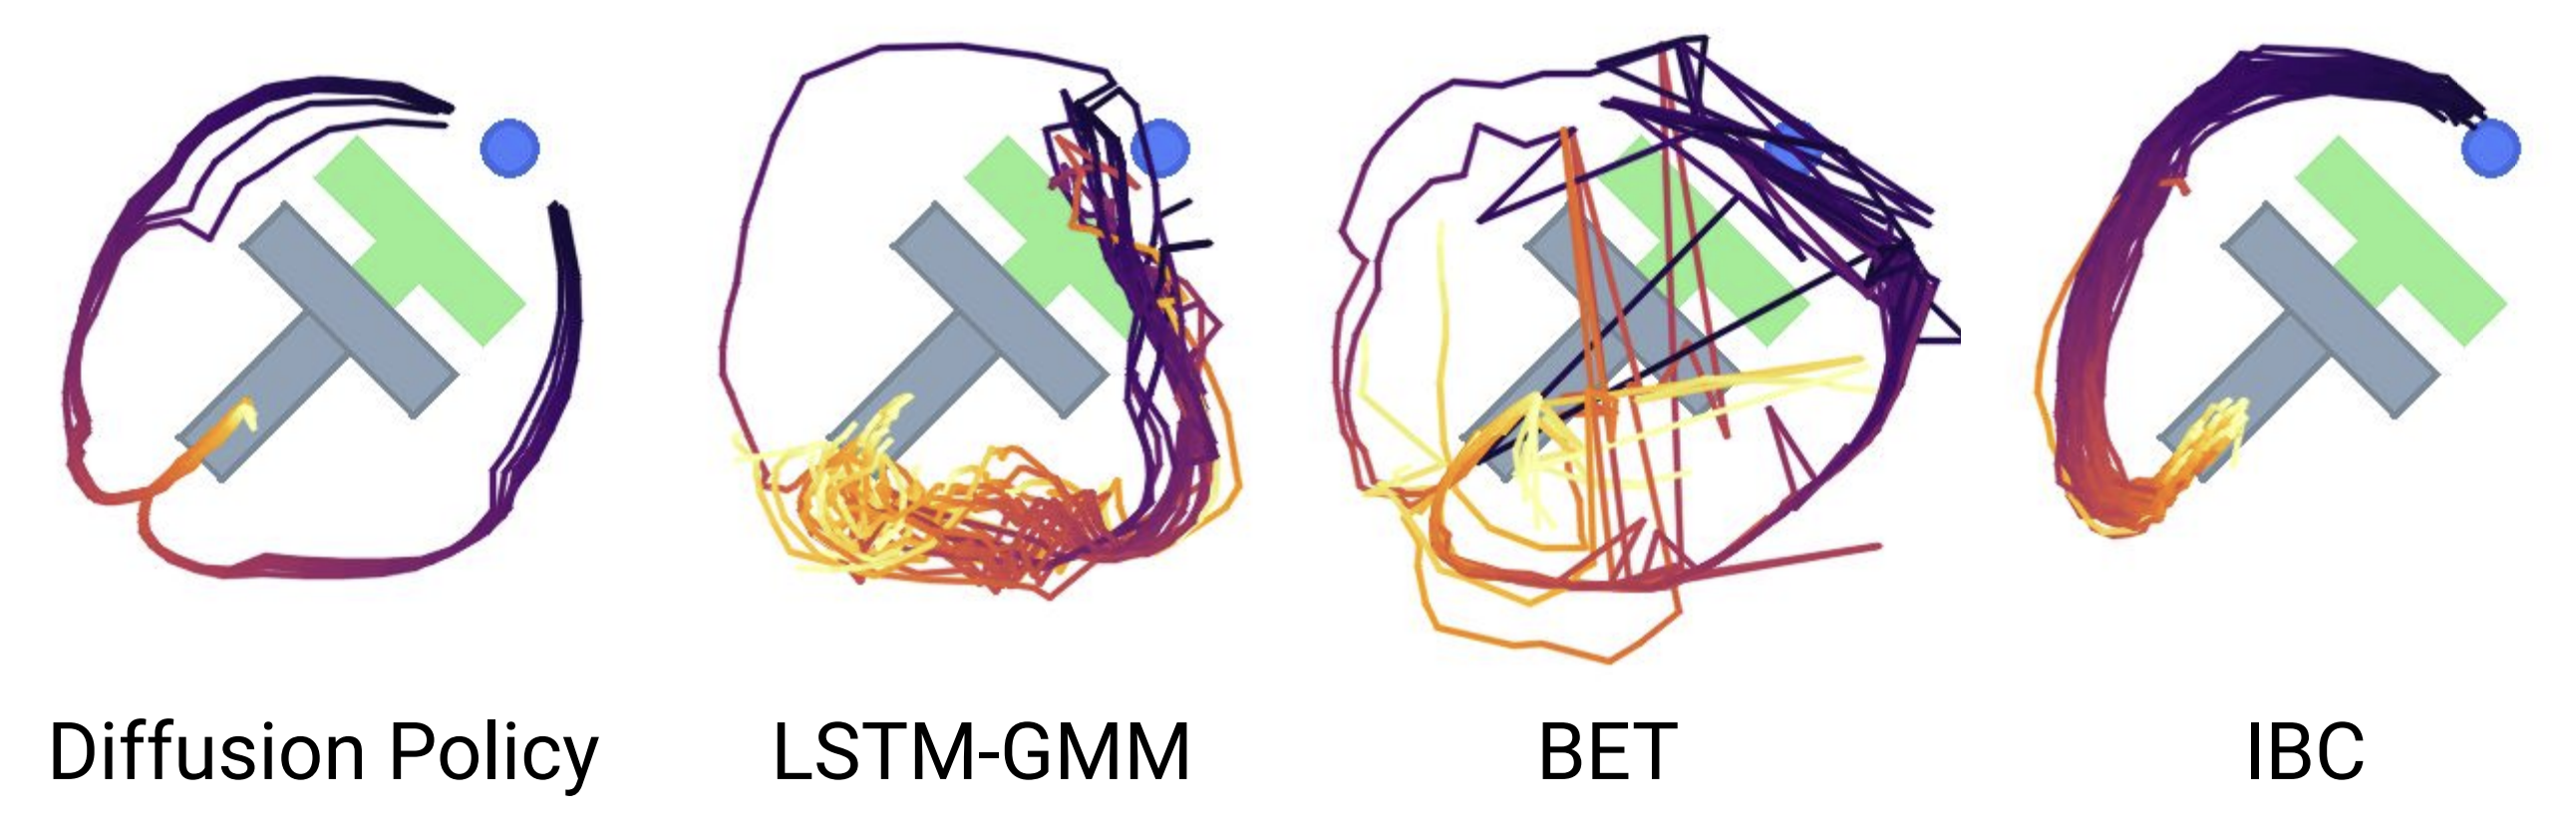
\includegraphics[width=0.95\textwidth]{./img/multimodal_beh.png}
    \end{center}
\end{frame}

\begin{frame}[t]{Robotic Control}
    Diffusion Policy with position control outperforms velocity-control
    \textbf{Reasoning}:
    \begin{itemize}[label=-]
        \item action multimodality more pronounced in position-control
        \item position control suffers less from compounding errors than velocity control
    \end{itemize}
    \begin{center}
        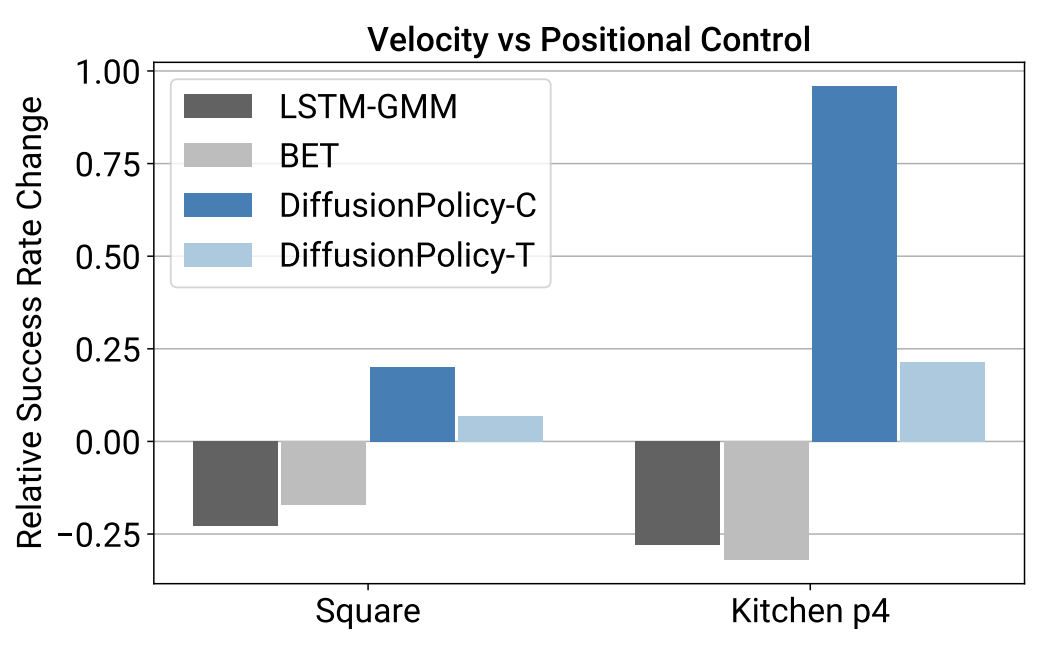
\includegraphics[width=0.7\textwidth]{./img/control_cmp.png}
    \end{center}
\end{frame}

\begin{frame}[t]{Benefits of Action Prediction}
    % IBC struggle in high-dimensional action space with non-smooth energy landscape
    % sequence predictions are avoided in policy learning bc difficult to sample
    \textbf{Temporal Action Consistency}: DDPM represents action in a high-dimensional action sequence overcoming:
    % IBC: Implicit BC: reformulate BC as composition of argmin action with continuous energy field
    \begin{enumerate}[label=\arabic*.]
        \item \textbf{Temporal Action Consistency}: Alternate approach (BC-RNN / BET) represents actions as independent multimodal distributions leading to jittery actions
        \item \textbf{Robustness to Idle Actions}: Single step policies overfit to pausing behavior (BC-RNN + IBC get stuck) % if idle actions not explicitly removed from training
        % cause the method to sample actions from different independent distributions 
    \end{enumerate}
    \begin{center}
        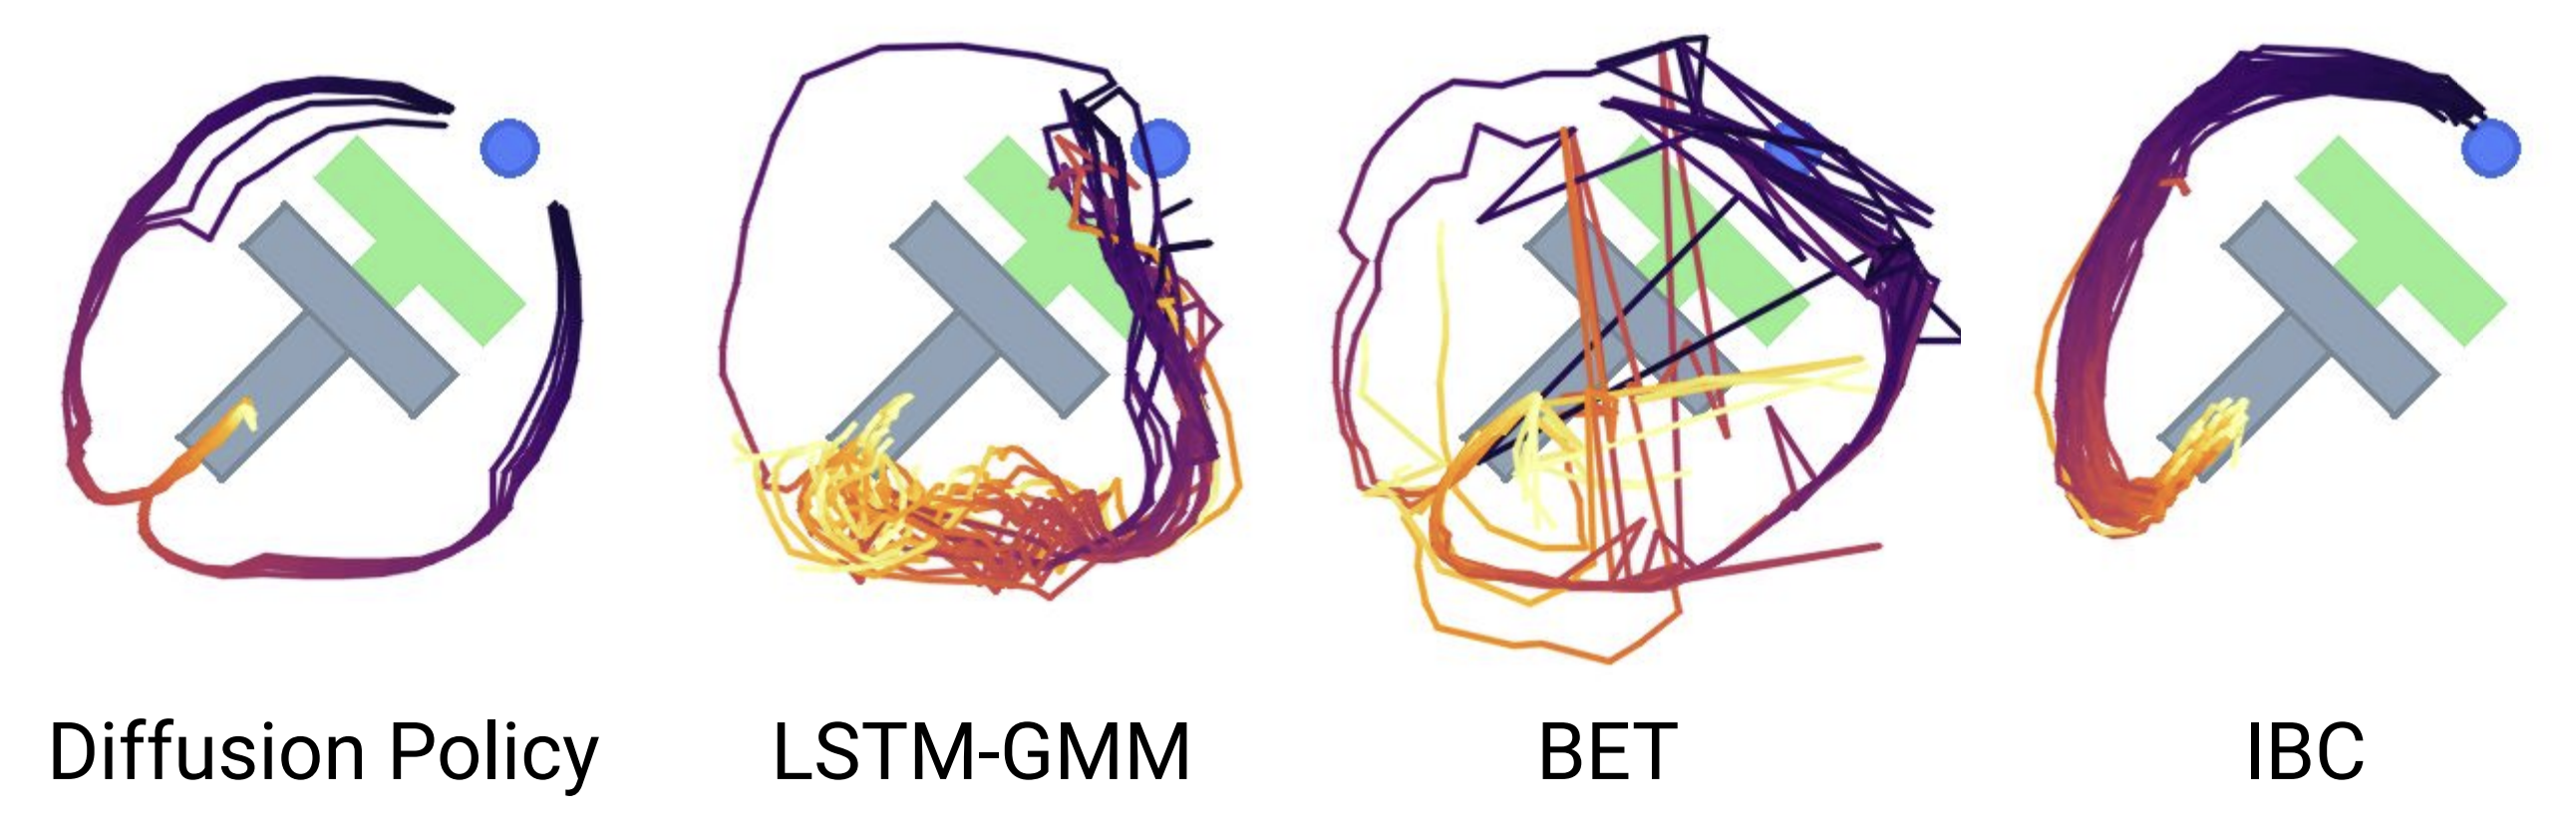
\includegraphics[width=0.7\textwidth]{./img/multimodal_beh.png}
    \end{center}
\end{frame}

\section{Key Findings}
\begin{frame}[t]{Diffusion Policy Benefits}
    Diffusion policy ...
	\begin{columns}
		\begin{column}{.5\textwidth}
    \begin{enumerate}[label=\arabic*.]
        \item expresses short and long-horizon multimodality
        % short horizon: multiple ways of achieving the same immediate goal from demo data
        % long horizon: completion of different sub-goals in inconsistent order
        \item better leverages position control
        \begin{itemize}[label=-]
            \item Baseline methods work better with velocity control
        \end{itemize}
        % having action horizon > 1 improves policy + consistent actions and compensate for idle portions
        \item has a better action horizon tradeoff
        \begin{itemize}[label=-]
            \item Horizon $>$ 1 help policy predict consistent actions 
            \item Compensate for idle portions
            \item Optimal action horizon of 8 steps
        \end{itemize}
    \end{enumerate}
		\end{column}
		\begin{column}{.5\textwidth}
            \begin{center}
                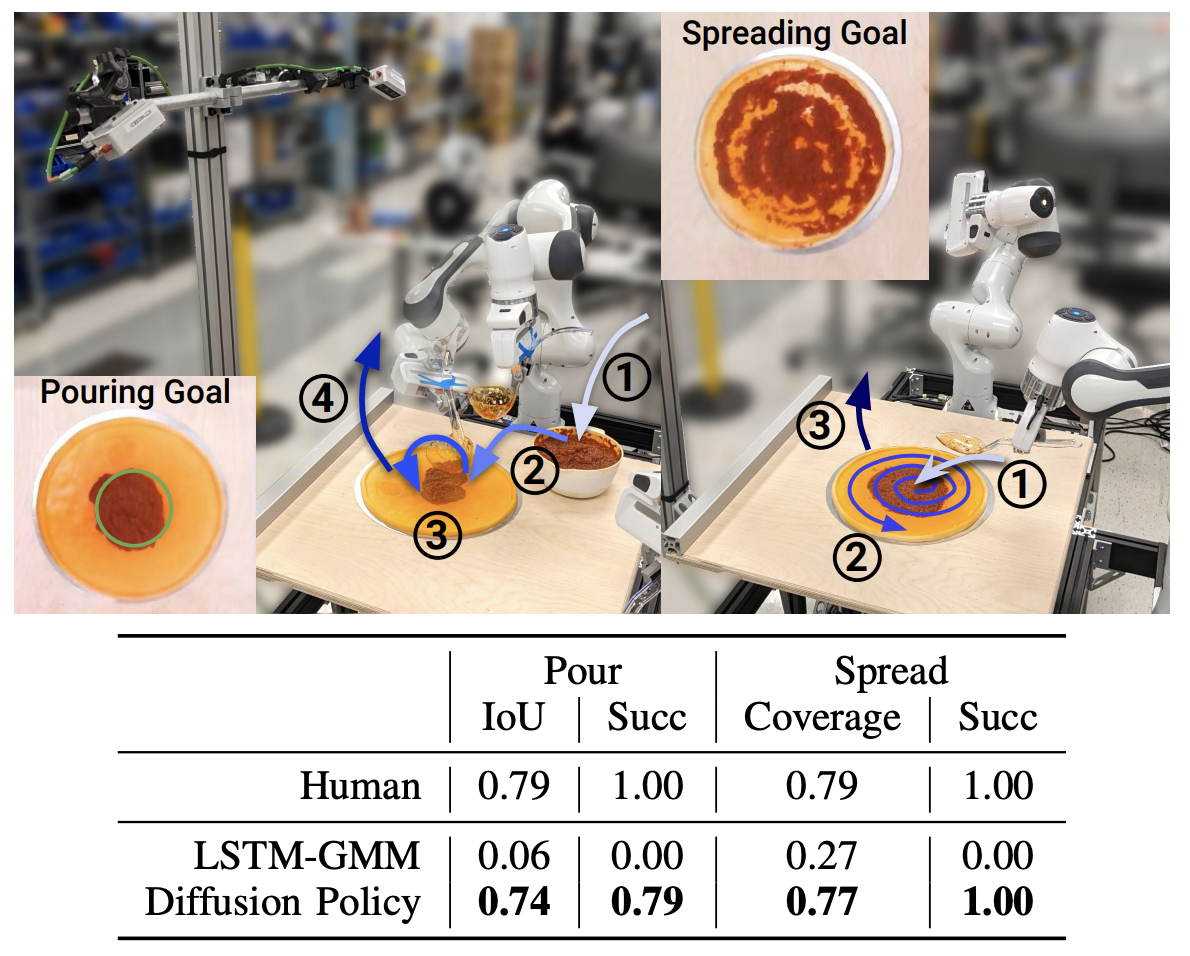
\includegraphics[width=\textwidth]{./img/real_world_diff.png}
            \end{center}
		\end{column}
	\end{columns}
\end{frame}

\begin{frame}{Thank you!}
	\begin{center}
        Have a great rest of your Day!!!
	\end{center}
	\begin{center}
		% \textbf{Slides:} {\small \url{https://cs.purdue.edu/homes/jsetpal/slides/dnc_by_agop.pdf}}
	\end{center}
\end{frame}

\end{document}